% !TEX root = msc_thesis.tex

\begin{figure}[tb]
	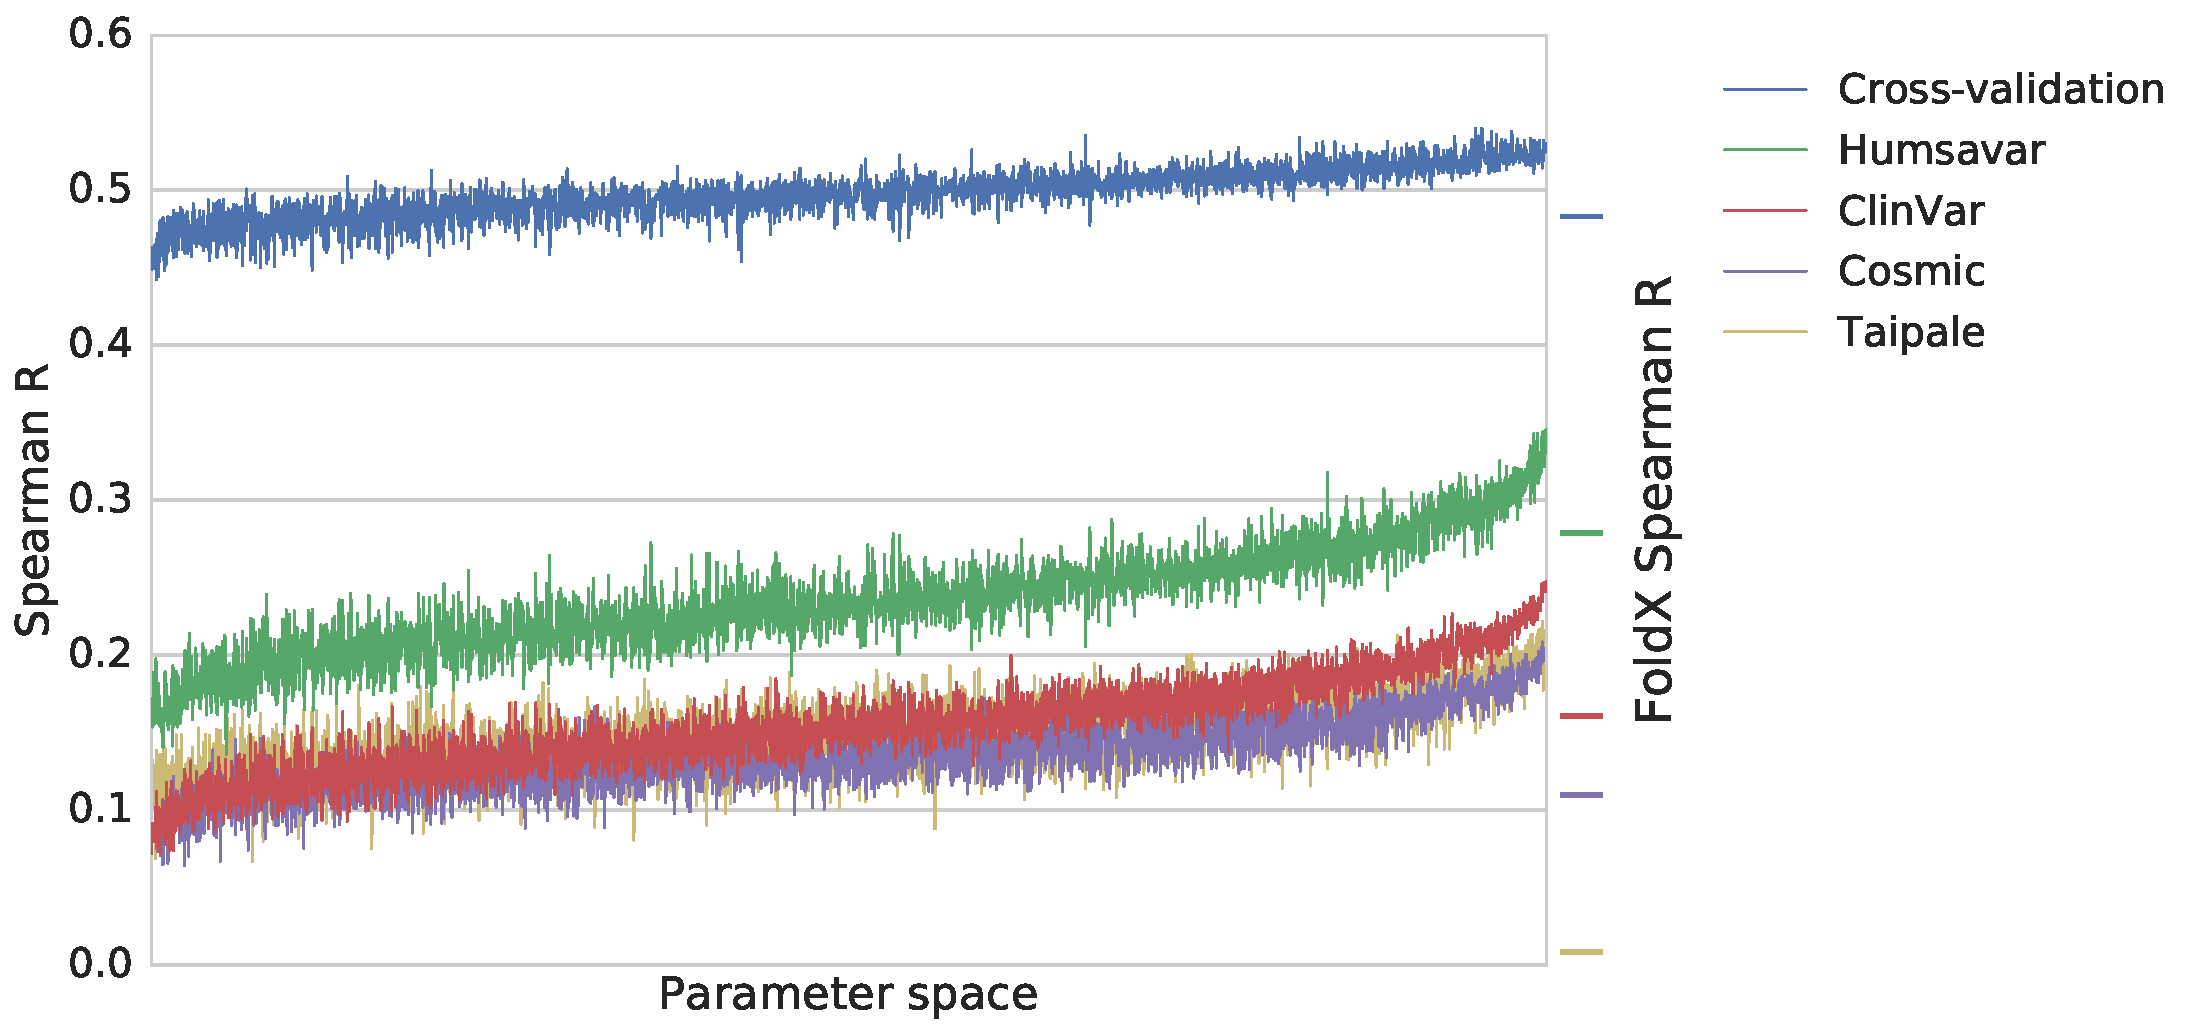
\includegraphics[width=0.9\linewidth]{static/elaspic_training_set/machine_learning/gridsearch_core.pdf}
	\caption[Core predictor hyperparameter optimization.]{
        Core predictor hyperparameter optimization.
        The combined score (black line) was calculated using Equation \ref{eq:combined_score_core}.
		We chose the set of hyperparameters that correspond to the predictor with the highest combined score.
    }
	\label{fig:gridsearch_core}
\end{figure}

\begin{figure}[tb]
	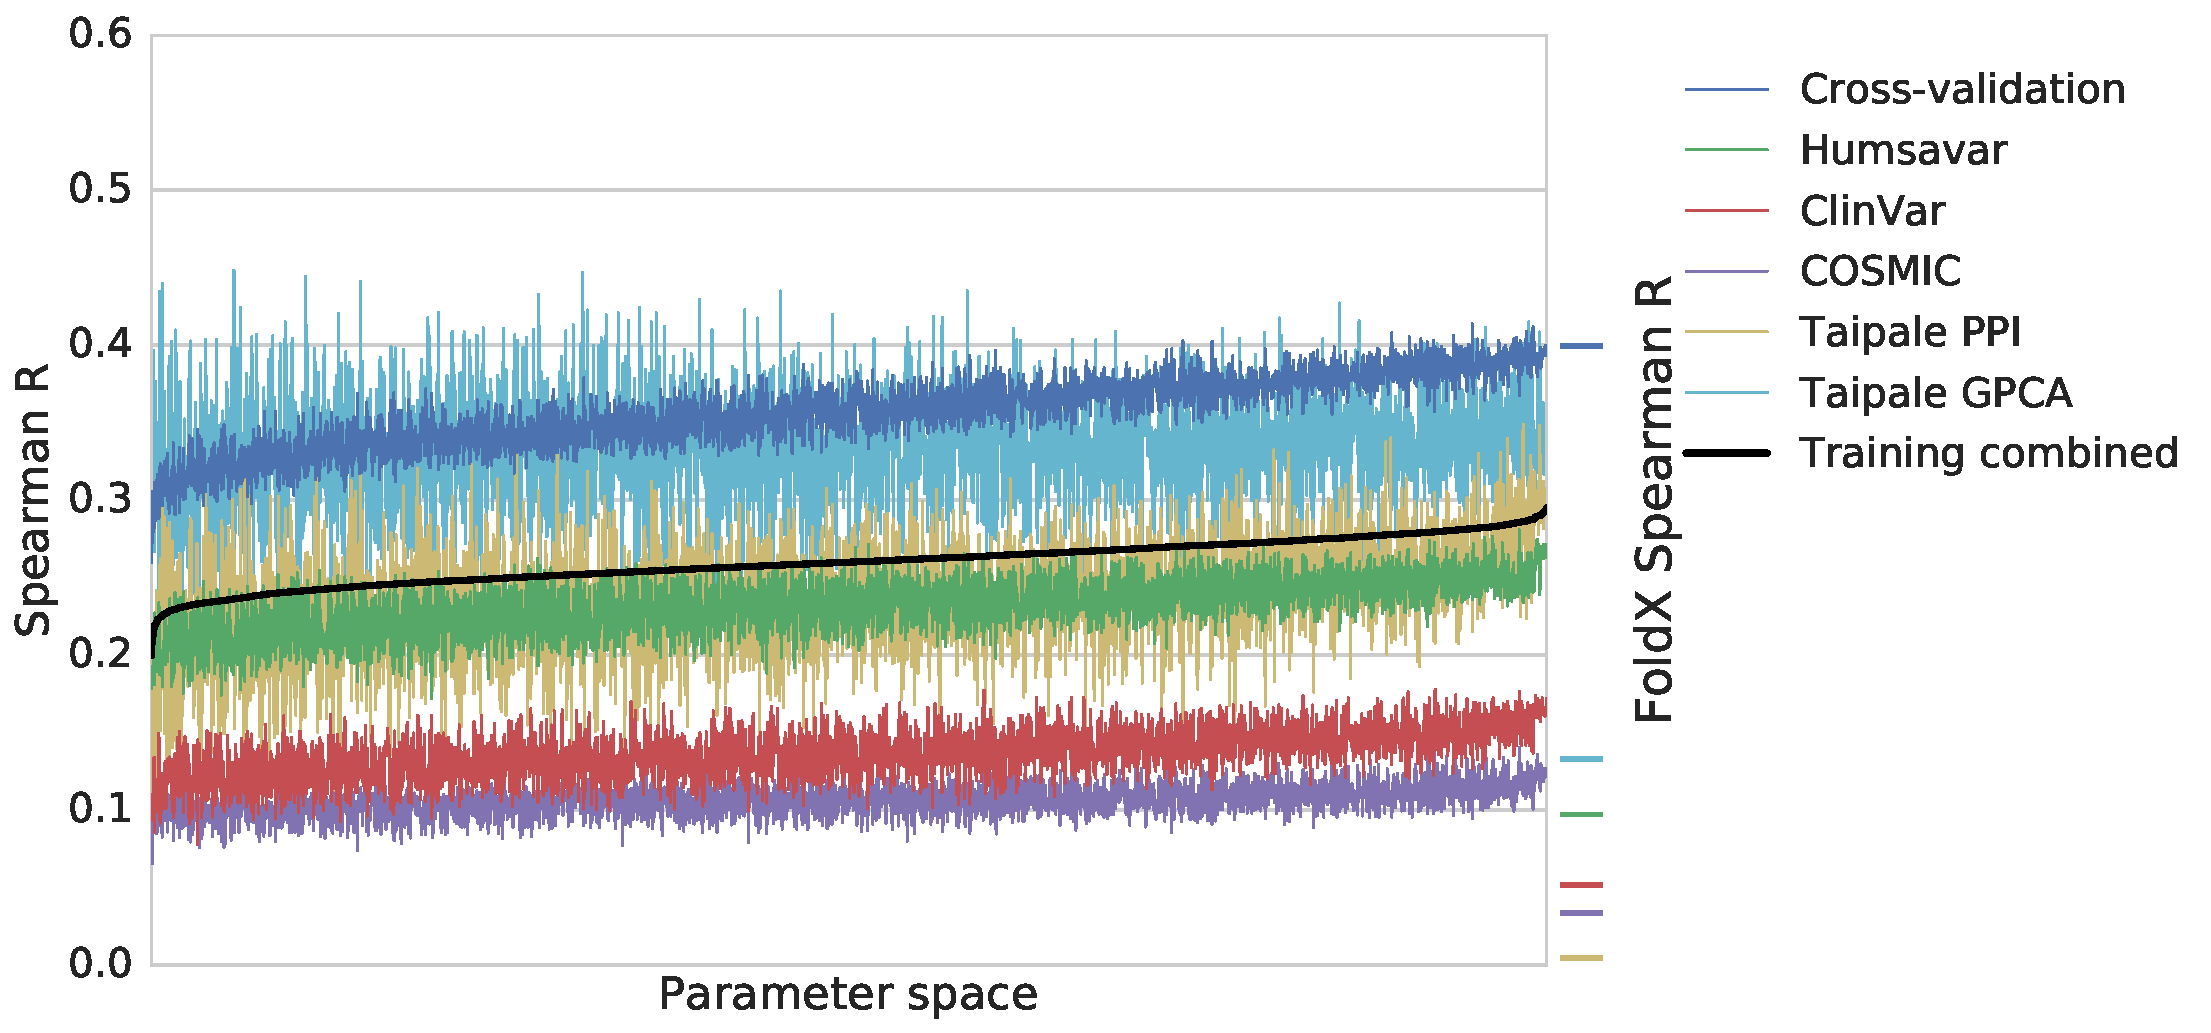
\includegraphics[width=0.9\linewidth]{static/elaspic_training_set/machine_learning/gridsearch_interface.pdf}
    \caption[Interface predictor hyperparameter optimization.]{
        Interface predictor hyperparameter optimization.
        The combined score (black line) was calculated using Equation \ref{eq:combined_score_interface}.
		We chose the set of hyperparameters that correspond to the predictor with the highest combined score.
    }
	\label{fig:gridsearch_interface}
\end{figure}

\clearpage

\begin{table}[tb]
    \captionsetup{width=0.6\textwidth}
	\centering
	\caption[Hyperparameter search space.]{
        Hyperparameter search space for tuning the gradient boosting regressor algorithm used in the core and interface predictors.
		An all-by-all combination of those hyperparameters was explored in order to find the sets of hyperparameters that produce the best-performing predictors.
    }
	\label{tab:gridsearch_parameters}
	\begin{tabular}{ l | l }
		\toprule
		Parameter name     & Parameter value                \\
		\midrule
		alpha              & 0.99, 0.95, 0.9, 0.8, 0.7, 0.5 \\
		learning\_rate     & 0.1, 0.05, 0.02, 0.01          \\
		loss               & huber                          \\
		max\_depth         & 10, 8, 6, 4                    \\
		max\_features      & 1.0, 0.8, 0.5, 0.3, 0.1,       \\
		min\_samples\_leaf & 29, 21, 17, 13, 9, 5, 3        \\
		n\_estimators      & 2000                           \\
		\bottomrule
	\end{tabular}
\end{table}

\begin{table}[tb]
	\centering
	\caption[Hyperparameters selected for the core predictor.]{
            Hyperparameters selected for the core predictor.
        }
    \label{tab:core_hyperparameters}
	\begin{tabular}{ l | l }
		\toprule
		Parameter name     & Parameter value \\
		\midrule
		alpha              & 0.5             \\
		learning\_rate     & 0.01            \\
		loss               & huber           \\
		max\_depth         & 4               \\
		max\_features      & 0.246           \\
		min\_samples\_leaf & 17              \\
		n\_estimators      & 2000            \\
		\bottomrule
	\end{tabular}
\end{table}

\begin{table}[tb]
	\centering
	\caption[Hyperparameters selected for the interface predictor.]{
            Hyperparameters selected for the interface predictor.
        }
	\label{tab:interface_hyperparameters}
	\begin{tabular}{ l | l }
		\toprule
		Parameter name     & Parameter value \\
		\midrule
		alpha              & 0.9             \\
		learning\_rate     & 0.01            \\
		loss               & huber           \\
		max\_depth         & 4               \\
		max\_features      & 0.3             \\
		min\_samples\_leaf & 13              \\
		n\_estimators      & 2000            \\
		\bottomrule
	\end{tabular}
\end{table}
